\documentclass[a4paper,12pt]{article}

\usepackage{amsthm}
\usepackage{amssymb}
\usepackage{amsmath}
\usepackage{hyperref}
\usepackage{xifthen}
\usepackage{xparse}
\usepackage{dsfont}
\usepackage{xcolor}

\usepackage{fullpage}

% Left-right bracket
\newcommand{\lr}[1]{\left (#1\right)}

% Left-right square bracket
\newcommand{\lrs}[1]{\left [#1 \right]}

% Left-right curly bracket
\newcommand{\lrc}[1]{\left \{#1\right\}}

% Left-right absolute value
\newcommand{\lra}[1]{\left |#1\right|}

% Left-right upper value
\newcommand{\lru}[1]{\left \lceil#1\right\rceil}

% Scalar product
\newcommand{\vp}[2]{\left \langle#1, #2 \right \rangle}

% The real numbers
\newcommand{\R}{\mathbb{R}}

% The natural numbers
\newcommand{\N}{\mathbb{N}}

% A nicer emptyset symbol
\let\emptyset\varnothing

% Set constructor
\newcommand{\setdef}[2]{\lrc{ #1 \; \text{\textbar} \; #2}}

% j'th entry
\newcommand{\xj}{X^{(j)}}

% eps, delta - dp
\newcommand{\edp}{$(\epsilon, \delta)$-DP}

% rando algo M
\newcommand{\M}{\mathcal{M}}

% Probability
\newcommand{\prob}[1]{\textnormal{Pr}\lrs{#1}}



\usepackage[utf8]{inputenc}
\usepackage{graphicx}  % For including images
\usepackage{bm}  % For bold math symbols

\usepackage{amsfonts}
\usepackage{todonotes}
\usepackage{hyperref}
\usepackage{cleveref}  % For referencing equations
\usepackage{cite} % For bibtex

% For writing todo inline
\presetkeys%
    {todonotes}%
    {inline}{}

% Used for writing pseudo code
\usepackage{algorithm}
\usepackage{algpseudocode}
% defined for writing input/output in pseudo code
\algblock{Input}{EndInput}
\algnotext{EndInput}
\algblock{Output}{EndOutput}
\algnotext{EndOutput}
\newcommand{\Desc}[2]{\State \makebox[6em][l]{#1}#2}

\usepackage[smartEllipses]{markdown}

\renewcommand\qedsymbol{$\blacksquare$}
\renewenvironment{proof}{{\textit{Proof} \\}}{\qed}

\newtheorem{definition}{Definition}[section]
\newtheorem{theorem}{Theorem}

\newtheorem{corollary}{Corollary}[section]
\newtheorem{lemma}{Lemma}[section]


\title{Differentially private vector aggreation in the case of multivariate gaussian data}
\author{Tim Sehested Poulsen}

\begin{document}

\maketitle
\todo{datasets -> dataset}
\todo{Write introduction, mention relation to average vector}
\section{Introduction}
In recent years there has been an increased focus on the privacy of individuals, as we live in the age of data.
More and more data is collected about us to be used for solving real world problems be that through old school statistics or 
advanced algorithmic systems, such as deep neural networks.
Often it is also the situation that to solve the problem at hand, sensitive data is required. 
In fact it is often the case that the more sensitive the data is the more useful it is.
Many attempts have been made to combat this dilemma, preserve the privacy of the individuals involved whilst harvesting the 
fruitful information which the sensitive data contains.
It has been shown repeatdatly  that de-anonymizing the data by removing "person-
ally identifiable information", such as names, PIN codes (Personal Identification Number) or the alike is not enough
to protect individuals from advesaries \cite{medical,netflix}. 
This project focuses releasing aggregate statistics from sensitive data to the public, which has also been shown to break privacy when released \cite{exposed}. \\

In an desire to mathematically define what is meant by privacy and giving a basis for algorithms to be compared and measured on their degree of privacy preservation 
the term \textit{Differential Privacy} was born. It is merely a mathematical definition (which will be covered shortly), but has been the golden standard on which
algorithms can be proofed against.
In essence it incapsulates that the effect of any individual on the output of a statistic,
 should be limited preferably to such an extend that the individual is not reckognizable.
As this project focuses on releasing the sum of vectors (with sensitive information) from a dataset, it specifically means in this setting
that it should, to some extend, not be possible to deduce whether any one individual was part of the calculated sum or not.
\todo{Why sums are important, its use cases and the relation to mean}

\section{Definitions \& Preliminaries}
Before I mathematically introduce the concept of Differential Privacy, there are some prerequistes in order to understand the definition.
Firstly I must introduce:

\textbf{The dataset} which will mostly be written as $X \in \R^{n \times d}$.
I have that $n$ denotes the number of entries in the dataset and 
$d$ is the number of dimensions of the dataset.
I will throughout the report refer to a single entry of 
the dataset as $x_i$ and dimension $j \in [d]$ of entry $i \in [n]$ as $x_{i,j}$.
I will also be using the notation $[n]$ which is the set $[n] = \{1,2,\dots,n-1, n\}$.
\vspace*{0.3cm}

\noindent The following two definitions are essential to the definition of differential privacy, and are used
when arguing about privacy and proving that an algorithm satisfies differential privacy.
\begin{definition}[Neighbouring dataset \cite{dwork2016}]
Two dataset $X, X' \in \R^{n \times d}$ are said to be 
neigbouring if they differ in at most a single entry.
Neighbouring dataset are denoted with the relation $X \sim X'$ and defined as followed
\[ X \sim X' \iff \lra{ \setdef{i \in \N}{i \le n \land x_i \ne x_i' } } \le 1 \]
\end{definition}

\begin{definition}[Sensitivity \cite{dpbasic}] % Definition 3.8
Let $f(X): \R^{n \times d} \rightarrow \R^k$ be a function. 
The $l_p$-sensitivity of $f$ is the maximal 
possible $l_p$-norm of the difference between the output of $f$ 
on two neighbouring dataset.
We denote the sensitivity as 
\[
\Delta_p (f) = \max_{X \sim X'} \| f(X) - f(X') \|_p 
\]
and then the total $l_2$-sensitivity is then
\end{definition}
\noindent Throughout the report I will only be working with $l_2$-sensitivity and
will just denote this as $\Delta(f)$ for ease of notation. \\

Differential privacy has multiple slightly different
formal definitions, all of which are very similair and there exists ways of
defining one of them in terms of another.
I will be working with the most standard on which is called $(\epsilon, \delta)$-Differential Privacy,
refered to as \edp.
\vspace*{0.3cm}
\begin{definition}[$(\epsilon, \delta)$-Differential Privacy \cite{dwork2016}]

A randomized algorithm $\M: \R^{n \times d} \rightarrow \mathcal{R}$ 
is $(\epsilon, \delta)$-differentially private if for all possible 
subsets of outputs $S \subseteq \mathcal{R}$ and all pairs of 
neighbouring dataset $X \sim X'$ we have that
\[ \prob{M(X) \in S} \le e^{\epsilon} \cdot \prob{M(X') \in S} + \delta \]

\end{definition}

\noindent The definition of differential privacy lends itself to posses some very useful properties.
I will cover two of these, which are of importance to this project.

\begin{lemma}[ \edp under post-processing \defcite{dpbasic}{Proposition 2.1}] %Proposition 2.1 in the cite
\label{lem:PostProc}

Let $\M: \R^{n \times d} \rightarrow \mathcal{R}$ be an $\ed$-differentially private 
algorithm. Let $f: \mathcal{R} \rightarrow \mathcal{R}'$ 
be an arbitrary randomized mapping, then 
$f \circ \mathcal{M}: \R^{n \times d} \rightarrow \mathcal{R}'$ is \edp.

\end{lemma}

\begin{proof}

Fix any pair of neighbouring datasets $X \sim X'$ and 
let $S \subseteq \mathcal{R}'$ be an arbitrary event. We then define 
$T = \setdef{r \in \mathcal{R}}{f(r) \in S}$.
We thus have that
\begin{align*}
    &\prob{f(\mathcal{M}(X)) \in S} = \prob{\mathcal{M}(X) \in T} \\
    &\le e^{\epsilon} \cdot \prob{\mathcal{M}(X') \in T} + \delta = 
    e^{\epsilon} \cdot \prob{f(\mathcal{M}(X')) \in S} + \delta
\end{align*}
    
\end{proof}



\begin{lemma}[\edp under composition \defcite{dpbasic}{Theorem 3.16} ] % Theorem 3.16
Let $\mathcal{M}_i: \R^{n \times d} \rightarrow \mathcal{R}_i$ be an $\lr{\epsilon_i, \delta_i}$-differentially private algorithm
for $i \in [k]$. Then if $\mathcal{M}_{[k]} : \R^{n \times d} \rightarrow \prod_{i=1}^{k} \mathcal{R}_i$ is defined to be
$\mathcal{M}_{[k]} = \lr{\mathcal{M}_1(X), \mathcal{M}_2(X), \dots, \mathcal{M}_{k}(X)}$ then we have that
$\mathcal{M}_{[k]}$ is $\lr{ \sum_{i \in [k]} \epsilon_i , \sum_{i \in [k]} \delta_i }$-differentially private.
\end{lemma}
\noindent The proof is a bit long and is omitted here, but can be found in Appendix B of \cite{dpbasic}.



\paragraph{Error Measure}
As this report concerns itself exclusively with the sum of entries 
in a dataset, error will be defined as the expected
squared $l_2$-norm between the true sum and 
the output of a randomized algorithm.
So let $X \in \R^{n \times d}$ be the dataset and
$f(X) = \sum_i^n x_i$ be the true sum of all entries. The error of a
randomized algorithm $M : \R^{n \times d} \rightarrow \R^d$
which estimates $f(X)$ is then 
\[
    \text{Err}(M) := \ee{M(X) - f(X)}
\]

\paragraph{extra}

\subsection{Quadratic forms of random variables}
\todo{write cohesive text here, and decide what to keep}

\begin{lemma}
\label{lem:GaussTrans}
Let $X \sim \mathcal{N}(\mu, \sigma^2)$ be a gaussian random variable and let $r \in \R$ be a constant.
We then have that
\begin{align*}
    &rX \sim \mathcal{N}(\mu, (r\sigma)^2) \\
    &X - r \sim \mathcal{N}(\mu-r, \sigma^2) 
\end{align*}
    
\end{lemma}

Quadratics of random variables have been well studied \cite{BatesQuadForm,MathaiQaudForms}, 
specially in the case of multivariate gaussian varaibles \cite{IowaQuadNormForms,MathaiQaudForms}.
Even more research has been done in evaluating the CDF of these quadratic forms
for Gaussian random vectors \cite{QuadFormsNume,QaudFormsBounds}.

\begin{lemma}[Expectation of a quadratic random variable \cite{BatesQuadForm}]
\label{lem:ExpQuad}
Let $X$ be a $d$-dimensional random vector with expected value $\Exp{X} =  \bm{\mu_{X}}$
and covariance matrix $\var{X} = \bm{\Sigma_{X}}$. Let also $A$ be a constant 
$d \times d$ symmetric matrix, then 
\[
    \Exp{X^T A X} = tr \lr{A \bm{\Sigma_X}} + \bm{\mu}^T A\bm{\mu}
\]
\end{lemma}

\begin{proof}
Blah blah
\begin{align*}
    &\Exp{X^T A X} 
    =\text{tr}\lr{\Exp{X^T A X}} 
    =\Exp{\text{tr} \lr{X^T A X}} \\
    &= \Exp{\text{tr} \lr{A X X^T}}
    = \text{tr} \lr{A \Exp{X X^T}} 
    = \text{tr} \lr{A \lr{ \var{X} + \bm{\mu} \bm{\mu}^T}} \\
    &= \text{tr} \lr{A \bm{\Sigma}} + \text{tr} \lr{A \bm{\mu \mu^T}}
    = \text{tr} \lr{A \bm{\Sigma}} + \bm{\mu}^T A \bm{\mu}
\end{align*}
blah
\end{proof}
\begin{corollary}
\label{cor:expNorm}
Let $X \sim \mathcal{N}(\bm{0}, \bm{\Sigma_X})$ be a $d$-dimensional gaussian vector
with expected value $\bm{0}$, and let $\sigma_j^2$ denote the variance of the 
$j$'th dimension where $1 \le j \le d$.
By lemma \ref{lem:ExpQuad} we have that the expected $l_2$-norm 
of such a vector is given by
\[
    \ee{X} = \text{tr} (\bm{\Sigma_X}) = \sum_{j=1}^d \sigma_j^2
\]
\end{corollary}


\section{Algorithms}
\subsection{The Gaussian Mechanism}
One of the most fundamental algorithms for achieving 
\edp is the Gaussian Mechanism \cite{dpbasic}. It computes the real
value of a statistic, where the $l_2$-sensitivity is known.
That is it produces a \edp estimate of a function 
$g: \R^{n \times d} \rightarrow \R^{d}$ where the $l_2$-sensitivity $ \Delta(g) $ 
is known.
It does so by computing the value of $g(X)$ and then adding noise
to each dimension drawn from the normal distribution 
$\mathcal{N}(0, \sigma_{\epsilon,\delta}^2)$.
This can be seen as adding a noise vector $\eta$ which 
is then distributed according to
the multivariate normal distribution 
$\mathcal{N}(\bm{0}, \sigma_{\epsilon,\delta}^2I)$. 
Pseudo code for the algorithm can be seen in Algorithm \ref{alg:gaussmech}.

\begin{algorithm}
\caption{The Gaussian Mechanism}\label{alg:gaussmech}
\begin{algorithmic}
    \Input
    \Desc{$\sigma_{\epsilon,\delta}$}{Standard deviation required to achieve \edp}
    \Desc{$X \in \R^{n \times d}$}{Dataset}
    \EndInput
    \Output
    \State\edp estimate of $g(X)$
    \EndOutput
    \For{$j \in [d]$}
        \State$\eta_j \gets \textnormal{sample from } \mathcal{N}(0, \sigma_{\epsilon,\delta}^2)$
    \EndFor \\
    \Return$g(X) + \bm{\eta}$
\end{algorithmic}
\end{algorithm}
\noindent The algorithm quite intuitively prodcues error which is purely given by the norm of the noise added, and the expected error can be calculated to be
\[
    \ee{(g(X) + \bm{\eta}) - g(X)} = 
    \ee{\bm{\eta}}
\]
Which by corollary \ref{cor:expNorm} is 
\begin{equation}
\label{eq:ExpErrGM}
    \ee{\eta} = \sum_i^d \sigma_{\epsilon,\delta}^2 = d \cdot \sigma_{\epsilon,\delta}^2
\end{equation}
It is apparent that the main difficulty of the mechanism 
lies in determining a $\sigma_{\epsilon, \delta}$ which achieves
\edp, and preferably the smallest such one.

The following theorem was initially proven
\begin{theorem}\textnormal{\cite{dpbasic}}
\label{theo:gaussMech}
Let $g: \R^{n \times d} \rightarrow \R^{d}$ be an arbitrary 
$d$-dimensional function with $l_2$-sensitvity 
$ \Delta(g) = \max_{X \sim X'} \| g(X) - g(X') \|$, 
and let $\epsilon \in (0,1)$.
The Gaussian Mechanism with
$\sigma_{\epsilon, \delta} = \Delta(g)  \sqrt{2\ln(1.25/\delta)}/\epsilon$ 
is \edp.
\end{theorem}
The proof is rather long and is therefore ommitted here. A few years later it was shown in \cite{BalleWang} how to compute the minimal $\sigma_{\epsilon, \delta}$.
\begin{theorem}\textnormal{\cite{BalleWang}}
\label{theo:OptSig}
The Gaussian Mechanism is differentially private if and only if $\sigma_{\epsilon, \delta} \ge \Delta(g) \cdot \sigma_{opt}$ where
$\sigma_{opt} \in \R$ is the smallest value greater than 0, which satisfies
\begin{equation}
\label{eq:sigopt}
    \Phi \lr{\frac{1}{2\sigma_{opt}} - \epsilon\sigma_{opt}} - e^{\epsilon} \Phi \lr{-\frac{1}{2\sigma_{opt}} - \epsilon\sigma_{opt}} \le \delta
\end{equation}
\end{theorem}
In \cite{BalleWang} it is also shown how to compute this value, but since this is of no importance to this project it will therefore not be covered here.
For the rest of the report I will only be referring to $\sigma_{opt}$ as the minimal value given by equation \eqref{eq:sigopt}.

The main downside of the Gaussian Mechanism is that it adds equal noise to all dimensions, regardless of the sensitivity in that dimension.
As this report focuses on giving differentially private estimates of sums of vectors, it is natural to ask whether adding equal noise in all dimensions
is optimal in this setting. Let us define the function of interest $f(X) = \sum_{i \in [n]} x_i$, for a dataset $X \in \R^{n \times d}$. 
The sensitivity of this function must be twice the largest possible norm of any vector.
Therefore if the largest difference between any two neighbouring datasets 
in the $j$'th dimension can be limited as follows
\begin{equation}
\label{eq:DimCon}
    \Delta_j := \max_{X \sim X'}|X^{(j)} - X'^{(j)}|
\end{equation}
and we say that $X$ and $X'$ differ in the $i$'th entry we conclude that
\begin{equation}
\label{eq:DelF}
    \Delta(f) = \max_{X \sim X'} \| f(X) - f(X') \| = 
    \max_{X \sim X'} \| x_i - x_i' \| = \sqrt{\sum_{j \in [d]} \Delta_j^2} = \|\bm{\Delta}\|
\end{equation}
where $\bm{\Delta} = (\Delta_1, \Delta_2, \dots, \Delta_d)$.

\noindent This means that by equation \ref{eq:ExpErrGM} the expected error of the Gaussian Mechanism when estimating $f(X)$ is given by
\begin{equation}
\label{eq:GMErr}
    \ee{\eta} = d \cdot \sigma_{\epsilon, \delta}^2 = d \cdot \lr{\Delta(f) \cdot \sigma_{opt}}^2 =
    d  \cdot \sigma_{opt}^2 \cdot \| \bm{\Delta} \|^2 
\end{equation}
A logical next step would be to add noise to each dimensions such that it is proportional to the sensitivity of that dimension.
This has been studied in \cite{Lebeda2022} and lays the foundation for this report. Their mechanism, appropriately called the Elliptical Gaussian Mechanism
works very similairly to the Gaussian Mechanism as described by algorithm \ref{alg:gaussmech}, though instead of sampling all $\eta_j$ from 
$\mathcal{N}(0,\sigma_{\epsilon, \delta}^2)$, here they are instead drawn from $\mathcal{N}\lr{0,\lr{\sigma_{opt}\cdot \frac{\Delta_j}{b_j}}^2}$. 
The algorithm is described in detail in Algorithm \ref{alg:EllipGM}

\begin{algorithm}
\caption{The Elliptical Gaussian Mechanism}\label{alg:EllipGM}
\begin{algorithmic}
    \Input
    \Desc{$\sigma_{opt}$}{Standard deviation as defined by theorem \ref{theo:OptSig}}
    \Desc{$X \in \R^{n \times d}$}{Dataset}
    \Desc{$\bm{b} \in \R^{d}$}{Scaling vector, where $\|\bm{b}\| = 1$}
    \Desc{$\bm{\Delta} \in \R^{d}$}{Sensitivies of all dimensions}
    \EndInput
    \Output
    \State \edp estimate of $f(X) = \sum_{i \in [n]} x_i$
    \EndOutput
    \For{$j \in [d]$}
        \State $\sigma_j \gets \sigma_{opt} \cdot \frac{\Delta_j}{b_j}$
        \State $\eta_j \gets \textnormal{sample from } \mathcal{N}(0, \sigma_j^2)$
    \EndFor \\
    \Return $f(X) + \eta$
\end{algorithmic}
\end{algorithm}

Though the algorithm seems short and simple, as the the only thing which distinguishes it from The Gaussian Mechanism 
is to draw samples from $\mathcal{N}(0, \lr{\sigma_{opt} \cdot \frac{\Delta_j}{b_j}}^2)$, 
it can be seen as a transformation of space. Consider transforming the data by the factor $\frac{b_j}{\Delta_j}$ in each dimension. 
Then you would have that each dimension is bounded
\[
    x_{i,j} \le \frac{\Delta_j}{2} \implies \widehat{x}_{i,j} := x_{i,j} \cdot \frac{b_j}{\Delta_j} \le \frac{b_j}{2}
\]
and in this space the sensitivity of $f(X)= \sum_{i \in [n]} x_i$ is then
\[
    \Delta(f) = \sqrt{\sum_{j \in [d]}\lr{\frac{b_j}{2} - \lr{-\frac{b_j}{2}}}^2} = \sqrt{\sum_{j \in [d]} b_j^2} = \|\bm{b}\| =  1
\]
This means that all points in $X$ are mapped to lie withing the unit ball, and in this space one can simply add noise to each 
dimension drawn from $\eta_j \sim \mathcal{N}(0, \sigma_{opt})$. Then the inverse transformation $\frac{\Delta_j}{b_j}$ 
can then be applied to each dimension of $f(\overline{X})$ as well as $\eta$, giving a differentially private estimate of $f(X)$, 
because differential privacy is preserved under post processing as per Theorem \ref{theo:PostProc}. \\


The main thing that really differentiates Algorithm \ref{alg:EllipGM} from the normal Gaussian Mechanism is the introduction of the scaling vector $\bm{b}$.
This is the scaling of how much weight should be attributed to each dimension when adding noise. It is shown how to determine the optimal values for $b_j$
in \cite{Lebeda2022}, and what the expected error of the mechanism then is.

\begin{theorem}[Optimality and error of the Elliptical Gaussian Mechanism \cite{Lebeda2022}]
The value for $b_j$ which minimizes the expected $l_2$ error $\ee{\bm{\eta}}$ of Algorithm \ref{alg:EllipGM} is as follows
\[
    b_j = \sqrt{\frac{\Delta_j}{\sum_{j \in [d]} \Delta_j}}
\]
which leads the error to be
\begin{equation}
\label{eq:EGMErr}
    \ee{\bm{\eta}} =  \sigma_{opt}^2 \cdot \| \bm{\Delta} \|_1^2
\end{equation}
where $\| \cdot \|_1$ is the $l_1$ norm.

\end{theorem}
The proof will be ommitted here, but it is very similair to the proofs for lemma \ref{lem:Optb} and Theorem \ref{theo:Alg3OptErr} which are in section \ref{seq:problem}.

Comparing the expected error between Algorithm \ref{alg:gaussmech} and Algorithm \ref{alg:EllipGM} we have the following ratio
\[
    \frac{d \cdot \sigma_{opt}^2 \cdot \| \bm{\Delta} \|^2 }{\sigma_{opt}^2 \cdot \| \bm{\Delta} \|_1^2} 
    = \lr{\frac{\sqrt{d}\| \bm{\Delta} \|}{\| \bm{\Delta} \|_1}}^2
    = \frac{d \sum_{j \in [d]} \Delta_j^2}{\lr{\sum_{j \in [d]} \Delta_j}^2}
\]
in which it can be seen that they are equal when all entries of $\bm{\Delta}$ are the same. Otherwise the error for the Elliptical Gaussian Mechanism is lower
when $\bm{\Delta}$ is skewed. As argued in \cite{Lebeda2022} Algorithm \ref{alg:EllipGM} improves Algorithm \ref{alg:gaussmech} by a factor in $[1,d)$.

\section{Problem setup}
\label{seq:problem}
As previously mentioned the problem investigated here consists of realeasing the sum of vectors 
in a dataset under differential privacy.
More formally we whish to release the value of 
$ f(X) = \sum_{i = 1}^n x_i  $
under \edp. \\
The common factor for achieving \edp in both the Gaussian Mechanism
and the Elliptical Gaussian Mechanism is the knowledge that data lie within some bounds.
Specifically for the Elliptical Gaussian Mechanism data is required to lie within some hyperrectangle.
It is formally described by equation \eqref{eq:DimCon} 
essentially saying that there is an upper and lower bound on each dimension.
This requirement is needed to know the $l_2$-sensitivity $ \Delta(f) $ as shown in equation \eqref{eq:DelF}.
In this project I will change this assumption and instead 
look at the case where each dimension is normally distributed.
This means that for each 
$ j \in [d] $ we have that 
$x_{i,j} \sim \mathcal{N}(\mu_j, \sigma_j^2)$.
An equivalent formulation is that the data is 
multivariately gaussianly distributed but with no correlation between dimensions.
This means that $x_i \sim \mathcal{N}(\bm{\mu}, \Sigma ) $, 
where $\Sigma$ is a diagonal matrix with the variance of each 
dimension along its diagonal.
It is quite apparent that determining a limit $ \Delta_j $ is impossible 
in this setting as the gaussian distribution is continously defined 
on the range $ (-\infty, \infty)$.
Several recent papers has combatted this by doing something called 
\textit{clipping} \cite{Huang2021,coinpress}. 
Clipping is the process of limiting all points to lie within a sphere with radius $C$.
To perform clipping two things are required, (1) a center of the sphere which we call $\bm{\hat{\mu}}$
which will become obvious why later, and (2) the radius $C$.
This means that every vector is transformed as such
\[
    \overline{x}_i := \mue + \min \lrc{\frac{C}{\| x_i - \mue \|}, 1} \cdot (x_i - \mue)
\]
Clipping entries by a factor $C$ thus means that $ \Delta(f) = 2C $ 
as any one entry cannot have more impact on the summation than $C$.
If the summation $f(X)$ is 
performed on a clipped dataset $\overline{X}$ it is equivalent to
defining the summation function $\overline{f}: \R^{n \times d} \rightarrow \R^d$ as
\[
    \overline{f}(X) = \sum_i^n \mue + \min \lrc{ \frac{C}{\| x_i - \mue \|}, 1} \cdot (x_i - \mue)
\]
Then by Theorem \ref{theo:OptSig} the 
gaussian mechanism with the function $\overline{f}$ is \edp with
$\sigma_{\epsilon, \delta} = \Delta\lr{\overline{f}} \sigma_{opt} = 2C \sigma_{opt}$.
Though the mechanism is still \edp it will now have 
a larger error when regarding the true sum
$f(X) = \sum_i^n x_i$ as the actual answer. If the probability of clipping is set
so low that we actually don't expect to clip any entries we can use $\overline{f}$ as an approximation of $f$.
Say there are $n$ points in a dataset, I will thus set the probability of clipping to be less than $\frac{1}{n}$ and get that
\[
    \ee{\lr{\overline{f}(X) + \eta} - f(X)} \approx \ee{\lr{f(X) + \eta} - f(X)} = \ee{\eta}
\]
This is of course not correct as some error will come from clipping points, but in this report 
I will solely focus on the error introduced by the noise added. Another source of error will come from
determining a good estimate for the center of the sphere, which optimally is $\mue = \bm{\mu}$, i.e. 
the mean of the distribution which the data originates from.
As lemma \ref{lem:dpcombine} states that \edp methods can be combined,
one can aquire such an estimate using some of the privacy budget.
However, doing so is in essence almost the same problem as I am attempting to solve.
The difference lies in the fact that this estimate could be given quite 
losely and I am interested in the sum (or mean) of a specific dataset not that of the original distribution. \\

In this setting, we again have the intuition that addding equal noise in all dimensions is non optimal, and instead the noise in a dimension should be proportional
to the variance $\sigma_j^2$ in that dimension. In a desire to achieve similair results to that of the Elliptical Gaussian Mechanism, just with normally distributed data,
I will use somewhat the same approach to achieve \edp.
They achieve \edp by finding scalings of each dimenion such that all points lie within a unit ball, i.e. a ball with radius $1$. 
There does not exist such a transformation for gaussian data, as there will always be a non-zero 
probability of observing points outside the unit ball.
Instead I will introduce the constraint that the expected squared distance betwwen any point and the estimated mean $\mue$ after the transformation should be $1$. 
I whish to find a scaling of each dimension $b_j$ s.t.
\begin{align}
    &\tilde{x}_i := (x_i - \mue) \odot \bm{b} \\
\label{eq:Alg3Con}
    &\ee{\tilde{x}} = 1
\end{align}
\todo{fix the rest, I mean introduce the estimated mean}
where $\bm{b} = (b_1, b_2, \dots, b_d)$, and $\odot$ is the element-wise product. 
Then $\overline{f}$ can be computed on this transformed dataset $\widehat{X}$, where the probability of clipping is less than $\frac{1}{n}$.
As Theorem \ref{theo:PostProc} shows, \edp is preserved under post processing, 
we can therefore add noise to each coordinate drawn from $\mathcal{N}(0,(2C\sigma_{opt})^2)$ in the transformed space to achieve \edp.
The transformation back to the original space is then done by multiplying each dimension with $b_j^{-1}$, and due to the linearity of transformation 
this is also done to the noise added.
We end up with the following noise vector being added
\[
    \bm{\eta} = \lr{ b_1^{-1}\eta_1, b_2^{-1}\eta_2, \dots, b_d^{-1}\eta_d }
\]
in which all $\eta_j \sim \mathcal{N}(0,(2C\sigma_{opt})^2)$, and then by lemma \ref{lem:GaussTrans} we have $b_j^{-1}\eta_j \sim \mathcal{N}(0, (b_j^{-1} \cdot 2C\sigma_{opt})^2)$.
The error introduced by the noise is then given by $\| \bm{\eta} \|^2$ and due to Corollary \ref{cor:expNorm} we have that the expectation of this error is 
\begin{equation}
\label{eq:Alg3Err}
    \ee{\bm{\eta}} = \sum_{j=1}^d \lr{b_j^{-1} \cdot 2C\sigma_{opt}}^2   = \lr{2C\sigma_{opt}}^2 \sum_{j=1}^d b_j^{-2}
\end{equation}

\begin{algorithm}
\caption{The Elliptical Gaussian Mechanism for Gaussian data}\label{alg:EGM2}
\begin{algorithmic}
    \Input
    \Desc{$\sigma_{opt} \in \R$}{Standard deviation as defined by Theorem \ref{theo:OptSig}}
    \Desc{$\bm{\sigma} \in \R^{d}$}{Standard deviations of all dimension}
    \Desc{$\bm{\hat{\mu}} \in \R^{d}$}{Differentially private estimate of the mean of all dimensions}
    \Desc{$X \in \R^{n \times d}$}{Dataset, where $x_{i,j} \sim \mathcal{N}(\mu_j,\sigma_j^2)$}
    \Desc{$\bm{b} \in \R^{d}$}{Scaling vector, s.t. $\ee{\lr{x_i - \bm{\hat{\mu}}} \odot \bm{b}} = 1$}
    \Desc{$p_C \in \R$}{Probability of clipping points}
    \EndInput
    \Output
    \State \edp estimate of $f(X)$
    \EndOutput
    \State $\widehat{\bm{\sigma}} \gets \bm{\sigma} \odot \bm{b}$
    \State $C \gets \textnormal{ Minimal $C$ satisfying } \prob{\|\widehat{x}\| > C} \le p_C \textnormal{, for } \widehat{x} \sim \mathcal{N}(\bm{0},\widehat{\bm{\sigma}})$
    \State $T \gets \bm{0}$
    \For{$i \in [n]$}
        \State $\widehat{x}_i \gets \lr{x_i - \bm{\hat{\mu}}} \odot \bm{b}$
        \State $T \gets T + \min \lr{\frac{C}{\|\widehat{x}_i\|}, 1} \cdot \widehat{x}_i + \bm{\hat{\mu}}$
    \EndFor
    \For{$j \in [d]$}
        \State $T_j \gets T_j \cdot b_j^{-1}$
        \State $\sigma_{\epsilon, \delta, j} \gets 2C\sigma_{opt} \cdot b_j^{-1}$
        \State $\eta_j \gets \textnormal{sample from } \mathcal{N}(0, \sigma_{\epsilon, \delta, j}^2)$
    \EndFor \\
    \Return $T + \bm{\eta}$
\end{algorithmic}
\end{algorithm}

The pseudo code for the mechanism is given in Algorithm \ref{alg:EGM2}. At first glance it seems quite different from Algorithm \ref{alg:EllipGM}
despite it being very similiar. The most notable thing here
is that the transformation has to be performed on the dataset,
as it is important which points are being clipped, in order to ensure that the mechanism is \edp.
In Algorithm \ref{alg:EllipGM} only the inverse transformation, $b_j^{-1}$, is being
applied on the noise to be added. \\

\noindent If we try to minimize the error introduced by the noise, we are back to a very similiar problem to the one solved in \cite{Lebeda2022}. 
Minimize the error described in equation \eqref{eq:Alg3Err}
under the constraint given in equation \eqref{eq:Alg3Con}.
The constraint can be given as
\begin{equation*}
    \ee{(x_i - \mue) \odot \bm{b}} = \sum_{j \in [d]} (b_j\sigma_j)^2 + \| \bm{\mu} - \mue \|^2 = 1
\end{equation*}
due to Corollary \ref{cor:expNorm}. We then relax this constraint by ommitting $\| \bm{\mu} - \mue \|^2$, 
as this in terms of the algorithm is constant and will simply lead to a constant scaling of all $b_j$.
Thus the constraint is
\begin{equation}
\label{eq:normcon}
\sum_{j \in [d]} (b_j\sigma_j)^2 = 1
\end{equation}

\noindent This leads to the following Lemma

\begin{lemma}
\label{lem:Optb}
Let $X \in \R^{n \times d}$ be a dataset where each dimension is independently gaussianly distributed, i.e.
$x_{i,j} \sim \mathcal{N}(\mu_j, \sigma_j^2)$.
Then the expected squared norm of the noise $\ee{\bm{\eta}}$, 
in Algorithm \ref{alg:EGM2} is minimized when
\[
    b_j = \frac{1}{\sqrt{\sigma_j} \sqrt{\sum_{i=1}^d \sigma_i}}
\]
\end{lemma}
\begin{proof}
Using lagrangian multipliers we find the local maxima or 
minia of the function subject to equality constraints.
To do so we construct the lagrangian function $\mathcal{L}: \R^{d+1} \rightarrow \R$ from the optimization problem given by
equation \eqref{eq:Alg3Err} and the constraint given by \eqref{eq:normcon} for ease of notation we define 
$\sigma_{\epsilon, \delta} := 2C\sigma_{opt}$.
\[
    \mathcal{L}(\bm{b},\lambda) = \sigma_{\epsilon,\delta}^2\sum_{j \in [d]} b_j^{-2}
    + \lambda \lr{ \sum_{j=1}^d \lr{\sigma_j b_j}^2 - 1}
\]
We then find the stationary points of it,
by setting the derivative of it to $\bm{0}$.
The derivative with respect to $b_j$ is 
\[
    \frac{\partial \mathcal{L}}{\partial b_j} (\bm{b}, \lambda)= 
    \frac{\partial}{\partial b_j} \lr{\sigma_{\epsilon,\delta}^2 \cdot b_j^{-2}
    + \lambda \lr{\sigma_j b_j}^2} =
    -2 \sigma_{\epsilon,\delta}^2 b_j^{-3} + 2 \lambda \sigma_j^2b_j
\]
I then solve $\frac{\partial \mathcal{L}}{\partial b_j}(\bm{b},\lambda) = 0$ for $b_j$
\begin{align}
    &-2\sigma_{\epsilon,\delta}^2 b_j^{-3} + 2 \lambda \sigma_j^2b_j = 0 \iff
    \lambda \sigma_j^2b_j = \sigma_{\epsilon,\delta}^2 b_i^{-3}  \\
\label{eq:solvbi}
    &\iff b_j^4 = \frac{\sigma_{\epsilon,\delta}^2}{\lambda \sigma_j^2} \iff 
    b_j = \frac{\sqrt{\sigma_{\epsilon,\delta}}}{\lambda^{\frac{1}{4}} \sqrt{\sigma_j}} 
\end{align}
I now have the last partial derivative 
$\frac{\partial \mathcal{L}}{\partial \lambda}(\bm{b},\lambda) = 0$ which I solve for
$\lambda$ using the previous expression for $b_j$.

\begin{align*}
    &\frac{\partial \mathcal{L}}{\partial \lambda}(\bm{b},\lambda) = 
    \sum_{j=1}^d \lr{ \sigma_j b_j}^2 - 1 \\
    &\sum_{j=1}^d \lr{ \sigma_j b_j}^2 - 1 = 0 \iff
    \sum_{j=1}^d \sigma_j^2 \lr{\frac{\sigma_{\epsilon,\delta}}{\sqrt{\lambda}\sigma_j}} = 1 \iff \\
    &\frac{\sigma_{\epsilon,\delta}}{\sqrt{\lambda}} \sum_{j=1}^d \frac{\sigma_j^2}{\sigma_j} = 1 \iff
    \sigma_{\epsilon,\delta} \sum_{j=1}^d \sigma_j = \sqrt{\lambda}
\end{align*}
Inserting back into equation \eqref{eq:solvbi}
\[
    b_j = \frac{\sqrt{\sigma_{\epsilon,\delta}}}{\lambda^{\frac{1}{4}} \sqrt{\sigma_j}} =
    \frac{\sqrt{\sigma_{\epsilon,\delta}}}{\sqrt{\sigma_{\epsilon,\delta} \sum_{i=1}^d \sigma_i} \sqrt{\sigma_j}} = 
    \frac{1}{\sqrt{\sigma_j} \sqrt{\sum_{i=1}^d \sigma_i} } 
\]
\todo{show that this stationary point is a minimum}
Giving us the value of $b_j$ which minimizes the expected error.
\end{proof}

Now to evaluate the expected error of the mechanism, which is given by equation \eqref{eq:Alg3Err}, it is highly important important to determine the value $C$.
As $C$ should be given by the minimal value which satisfies the inequality
\[
   \prob{ \| (x_i - \mue) \odot \bm{b} \| > C } = \prob{ \| (x_i - \mue) \odot \bm{b} \|^2 > C^2} < \frac{1}{n}
\]
again where $n$ denotes the number of points in the dataset.
As $x_i$ is a multivariate gaussian distribution, so is $(x_i - \mue) \odot \bm{b}$ by lemma \ref{lem:GaussTrans},
and it is the case that $\|(x_i - \mue) \odot \bm{b}\|^2$ is the sum of independent gaussian variables squared.
Such a sum is distributed as a generalized Chi-square \cite{GenChiSq}, and neither its PDF nor CDF has a closed form in the general case.
These quadratic forms of gaussian vectors has been studied well and for decades \cite{MathaiQaudForms}, and some special cases does have closed forms.
Some have also studied giving tail bounds on these probabilities \cite{QaudFormsBounds}, unfortunately there was none which were of use in this setting.
However, there does exist several numerical algorithms for evaluating the cumulative density function with high precision \cite{QuadFormsNume}. 
I would recommend using one of these algorithms in practice, and will do so in the emperical analysis in section \ref{sec:emperical}.
For the sake of analysis I will provide and upper bound on $C$ using Bernstein's inequality.

\begin{lemma}
\label{lem:Bernstein}
Let $X_1, X_2, \dots , X_d$ be $d$ independent random gaussian variables 
where for $ 1 \le j \le d$ we have that $X_j \sim \mathcal{N}(0, \sigma_j^2)$.
Let thereafter the largest standard deviation be denoted as $\sigma_* := \max_{j \in [d]} \sigma_j$,
we can then bound the probability for the sum of variables squared as follows 
\[
\prob{\sum_{j \in [d]} X_j^2  \ge 
    t \sqrt{8 \sum_{j \in [d]} \sigma_j^4} +
    \sum_{j \in [d]} \sigma_j^2 } < e^{-t^2}
\]
for
\[
0 \le t \le 
    \frac{1}{6 \sigma_*^2} \sqrt{2 \sum_{j \in [d]} \sigma_j^4}
\]
\end{lemma}
\begin{proof}
At first we define the random variable $Y_j = X_j^2 - \Exp{X_j^2}$ 
using the $j$'th gaussian random variable.
As $\Exp{Y_j} = \Exp{X_j^2 - \Exp{X_j^2}} = \Exp{X_j^2} - \Exp{X_j^2} = 0$ 
we have that $Y_j$ is zero centered. We are thus interested in giving bounds on
$\prob{\sum_{j \in [d]} Y_j}$. 
We can use Bernsteins inequality, if there exists some $L \in \R$ which satisfies 
\begin{equation}
\label{eq:BernCon}
    \Exp{ |Y^k_j| } \le \frac{1}{2} \Exp{Y_j^2} L^{k-2} k!
\end{equation}
for all $k \in \N$ with $k \ge 2$ and for all $j \in [d]$. \cite{wainwright_2019}

Initially we have that $\Exp{ |Y_j^k| } = \Exp{ |\lr{X_j^2 - \Exp{X_j^2}}^k|}$
and since $X_j^2 \ge 0$ and therefore also $\Exp{X_j^2} \ge 0$ 
we can therefore bound it by

\[
    \Exp{ |\lr{X_j^2 - \Exp{X_j^2}}^k|} \le \Exp{ | X_j^{2k} | } =
    \Exp{ | \lr{\sigma_j^2 Z}^{k} | } = 
    \sigma_j^{2k} \cdot \Exp{ |Z^{k} | }
\]
Where $Z \sim \chi^2_1$ is a chi square with 1 degree of freedom.
The moment generating function of $Z$ is 
$\Exp{Z^m} = 1 \cdot 3 \cdot 5 \cdot \ldots \cdot (2m - 1) $.
Using this we can get the following bound
\begin{align*}
    &\sigma_j^{2k} \cdot \Exp{ |Z^{k} | } =
    \sigma_j^{2k} \cdot \prod_{c=1}^k(2c-1) =
    \sigma_j^{2k} \cdot 3\cdot \prod_{c=3}^k (2c-1) \\
    &\le \sigma_j^{2k} \cdot 3 \cdot \prod_{c=3}^k 2c
    = \frac{3}{2}\sigma_j^{2k} \cdot 2^{k-2} \cdot k!
\end{align*}
Concluding that $\Exp{ |Y_j^k| } \le \frac{3}{2}\sigma_j^{2k} \cdot 2^{k-2} \cdot k!$.

\noindent Secondly I calculate $\Exp{Y_j^2}$ exactly to be used in equation \ref{eq:BernCon}
\begin{align}
\label{eq:ExpY2:1}
    &\Exp{Y_j^2} = 
    \Exp{\lr{X_j^2 - \Exp{X_j^2}}^2} \\
    &=\Exp{X_j^4 + \Exp{X_j^2}^2 - 2X_j^2\Exp{X_j^2}} \\
    &=\Exp{X_j^4} + \Exp{X_j^2}^2 - 2\Exp{X_j^2}^2 \\
    &=\Exp{X_j^4}  - \Exp{X_j^2}^2 =
    \sigma_j^4\Exp{Z^2}  - \lr{\sigma_j^2\Exp{Z}}^2 \\
\label{eq:ExpY2:2}
    &=3\sigma_j^4  - \sigma_j^4 =
    2\sigma_j^4
\end{align}

Equation \eqref{eq:BernCon} is therefore rewritten to 
\begin{align*}
    \frac{3}{2}\sigma_j^{2k} \cdot 2^{k-2} \cdot k! \le \frac{1}{2} \cdot 2 \sigma_j^4 L^{k-2} k! 
    \iff \frac{3}{2} \sigma_j^{2k-4} \cdot 2^{k-2} \le L^{k-2}
\end{align*}
This expression is then split into two cases, when $k=2$, in which it can be seen from equation \eqref{eq:BernCon} that this holds for any $L \in \R$.
The other case is $k>2$, where we have that 
\[
    \lr{\frac{3}{2}}^{\frac{1}{k-2}} \sigma_j^2 \cdot 2 \le L
\]

As $\lim_{k \rightarrow \infty} \lr{\frac{3}{2}}^{\frac{1}{k-2}} = 1$, 
and these constraints must hold for all $j \in [d]$, we can define $\sigma_* = \max_{j \in [d]} \sigma_j$ and finally have that
\begin{align*}
    &L = 3\sigma_*^2 
\end{align*}

We can then use Bernstein's inequality to bound the following 
\begin{equation}
\label{eq:BernIneq}
    \prob{\sum_{j \in [d]} Y_j \ge 2 t \sqrt{ \sum_{j \in [d]} \Exp{Y_j^2}}} < e^{-t^2}
\end{equation}

Which in in this case can be rewritten to get a tail bound on $\sum_{j \in [d]} X_j^2$,
by reusing results from equations \eqref{eq:ExpY2:1}-\eqref{eq:ExpY2:2}
\begin{align*}
&\prob{\sum_{j \in [d]} Y_j \ge 2 t \sqrt{ \sum_{j \in [d]} \Exp{Y_j^2}}} 
=\prob{\sum_{j \in [d]} \lr{X_j^2 - \Exp{X_j^2}} \ge 2 t \sqrt{ \sum_{j \in [d]} 2 \sigma_j^4}} \\
&=\prob{\sum_{j \in [d]} X_j^2  \ge 2 t \sqrt{ \sum_{j \in [d]} 2 \sigma_j^4} + \sum_{j \in [d]} \Exp{X_j^2}} 
=\prob{\sum_{j \in [d]} X_j^2  \ge 2 t \sqrt{ \sum_{j \in [d]} 2 \sigma_j^4} + \sum_{j \in [d]} \sigma_j^2}  \\
&=\prob{\sum_{j \in [d]} X_j^2  \ge 
    t \sqrt{ 8 \sum_{j \in [d]}  \sigma_j^4} +
    \sum_{j \in [d]} \sigma_j^2 } \\
\end{align*}

Finally giving us that 
\[
\prob{\sum_{j \in [d]} X_j^2  \ge 
    t \sqrt{ 8 \sum_{j \in [d]}  \sigma_j^4} +
    \sum_{j \in [d]} \sigma_j^2 } < e^{-t^2}
\]
as long as $t$ lies within the following bounds
\[
    0 \le t \le \frac{1}{2L} \sqrt{\sum_{j \in [d]} \Exp{Y_j^2}} =
    \frac{1}{6 \sigma_*^2} \sqrt{2 \sum_{j \in [d]} \sigma_j^4}
\]
\end{proof}

\noindent Combining lemma \ref{lem:Bernstein} with lemma \ref{lem:Optb} 
we have can conclude the following:

\begin{theorem}
\label{theo:Alg3OptErr}
Let $X \in \R^{n \times d}$ be a dataset in which all dimensions are independently gaussian random variables, i.e. $x_{i,j} \sim \mathcal{N}(\mu_j, \sigma_j^2)$. 
Let $\sigma_* := \max_{j \in [d]} \sigma_j$ be the maximal standard deviation of all dimensions. We then have that
when $\ln (n) \le \frac{\sum_{j \in [d]} \sigma_j^2}{18 \sigma_*^2}$ 
the expected squared error of the noise in algorithm \ref{alg:EGM2} can be upper bounded by 
\[
    \ee{\bm{\eta}} \le 4\sigma_{opt}^2  \cdot \sum_{j \in [d]} \sigma_j \cdot
    \lr{ \sqrt{8\ln(n) \sum_{i \in [d]} \sigma_i^2} + \sum_{j \in [d]} \sigma_j }
\]
when each $b_j$ is chosen according to lemma \ref{lem:Optb}.
\end{theorem}

\begin{proof}
By equation \eqref{eq:Alg3Err} the error is given by
\begin{equation}
\label{eq:Alg3Err2}
    \ee{\bm{\eta}} = \lr{2C\sigma_{opt}}^2 \cdot 
    \sum_{i=1}^d b_j^{-2} 
\end{equation}
We thus need to determine an upper bound for $C$, we begin by looking at the transformed data
when $\mue = \bm{\mu}$.
\begin{align*}
    &\tilde{x}_i := (x_i - \mue) \odot \bm{b} \textnormal{ , giving } \tilde{x}_{i,j} \sim \mathcal{N}\lr{0,\lr{b_j\sigma_j}^2} \\
    &\prob{ \| \tilde{x}_i \| \ge C} =
    \prob{ \| \tilde{x}_i \|^2 \ge C^2} =
    \prob{ \sum_{j \in [d]} \tilde{x}_{i,j}^2 \ge C^2}
\end{align*}

Which means I can give an upper bound on $C^2$, whilst having
$b_j \sigma_j = \sqrt{\frac{\sigma_j}{\sum_{i \in [d]} \sigma_i}}$ 
as the standard deviation.
Furthermore, I wish the clipping probability to be less than $n^{-1}$, giving me
\[
    e^{-t^2} = \frac{1}{n} \implies t = \sqrt{\ln (n)}
\]
Combining these results and using the upper bound on $C$ from lemma \ref{lem:Bernstein} I get the following
\begin{align*}
    C^2 &\le 2 \sqrt{\ln(n)} \sqrt{2\sum_{j \in [d]}  \lr{\lr{b_j\sigma_j}^4}} + 
    \sum_{j \in [d]} \lr{b_j\sigma_j}^2 \\
    &=\sqrt{8 \ln(n) \sum_{j \in [d]} \lr{\frac{\sigma_j}{\sum_{i \in [d]} \sigma_i}}^2} + 
    \sum_{j \in [d]} \frac{\sigma_j}{\sum_{i \in [d]} \sigma_i} \\
    &=\frac{\sqrt{8 \ln(n) \sum_{j \in [d]} \sigma_j^2}}{\sum_{i \in [d]} \sigma_i}
    + 1
\end{align*}
Inserting this back into equation \ref{eq:Alg3Err2} we conclude
\begin{align*}
    \ee{\bm{\eta}} &= 4\sigma_{opt}^2 \cdot 
    C^2 \cdot \sum_{i=1}^d b_j^{-2} \\
    &\le 4\sigma_{opt}^2 \cdot 
    \lr{\frac{\sqrt{8 \ln(n) \sum_{j \in [d]} \sigma_j^2}}{\sum_{i \in [d]} \sigma_i}
    + 1} \cdot \sum_{i=1}^d \lr{\sigma_i \cdot \sum_{j \in [d]} \sigma_j} \\
    &= 4\sigma_{opt}^2 \cdot 
    \lr{\frac{\sqrt{8 \ln(n) \sum_{j \in [d]} \sigma_j^2}}{\sum_{i \in [d]} \sigma_i}
    + 1} \cdot \lr{\sum_{i=1}^d \sigma_i}^2 \\
    &= 4\sigma_{opt}^2 \cdot \sum_{i=1}^d \sigma_i \cdot 
    \lr{\sqrt{8 \ln(n) \sum_{j \in [d]} \sigma_j^2}
    + \sum_{i=1}^d \sigma_i}
\end{align*}
And the constraint on $t = \sqrt{\ln (n)}$ from lemma \ref{lem:Bernstein} is
\begin{align*}
    &0 \le t \le \frac{1}{6 (b_j\sigma_*)^2} \sqrt{2\sum_{j \in [d]} (b_j\sigma_j)^4} \iff \\
    &\sqrt{\ln (n)} \le \frac{1}{6} \frac{\sum_{j \in [d]} \sigma_j}{\sigma_*} \sqrt{\sum_{j \in [d]} \lr{\frac{\sigma_j}{\sum_{i \in [d]} \sigma_i}}^2} \iff \\
    &\sqrt{\ln (n)} \le \sqrt{\lr{\frac{\sum_{j \in [d]} \sigma_j}{\sigma_*}}^2 \cdot \frac{2}{36} \cdot \sum_{j \in [d]} \lr{\frac{\sigma_j}{\sum_{i \in [d]} \sigma_i}}^2} \iff \\
    &\ln (n) \le \frac{1}{18\sigma_*^2} \cdot \sum_{j \in [d]} \sigma_j^2 \iff \\
    &\ln (n) \le \frac{\sum_{j \in [d]} \sigma_j^2}{18 \sigma_*^2}
\end{align*}
\end{proof}

At this point it would be preferable to compare the error of algorithm 3, to that of doing no transformation, and similairly deciding on a bound $C$ 
such that the clipping probability was less than $n^{-1}$ on $X$. However as I can only give upper bounds on these errors there is little to no value in comparing 
upper bounds as there is no guarentee on the thighness of these bounds. So even if I were to determine an upper bound for the error without transformation which was higher than that of algorithm 3, 
it could very well still be that the error was less in reality.
As previously mention, there exists numerical solutions for evaluating $\prob{\|x_i\| > C^2}$ so it is natural to perform an emperically evaluation of these errors
 and investigating whether the transformation lessen the error.
Intuitively it makes sense that allowing different noise to be added for each dimension, can only produce better results.
\todo{Write and discuss restrictiveness of the bound}
\todo{Write about alternative ways of giving upper bound on $C$, and why it is not so important}
\todo{Write alternative ways of defining the problem. CLip prob less than $n^{-1}$ and such}



\todo{Write emperical evaluation section} 
\section{Emperical Evaluation}
\label{sec:emperical}
For the emperical evaluation I wanted to investigate the 
improvement by calculating the expected error on hypothetical datasets. 
This is as a contrast to using real world datasets, where it is uncertain whether
the data is distributed according to a multivariate gaussian mechanism with independent dimensions.
Secondly I gain the benefit of creating a wide range of hypothetical scenarios and evaluating these.
When creating hypothetical dataset I am merely interested in the standard deviations of each dimension,
thus there is no need to truly create a dataset but instead I chose to 
synthetically create the parameters of a hypothetical dataset.
So I chose to have the standard deviation of each dimension be chosen according 
to Zipf's law \cite{zipf}. The distribution is often used to describe 
sizes of cities or frequencies of words in texts, but it can also be used to 
describe discrete distributions with different levels of skewness. 
This propoerty is what I will be utilizing, as I will chose the 
standard deviation of dimension $i \in [d]$ as
\[
    \sigma_i = \frac{ \frac{1}{i^\alpha}}{\sum_{j \in [d]} \frac{1}{j^\alpha}}
\]
The parameter $\alpha$ thus decides the skewness of how much each dimension contributes to the total amount of variance.
Figure \ref{fig:skew} shows how much each dimension contributes to the total variance for
$\alpha \in \{0.1,1,3\}$ and $d = 100$. This means that for high $\alpha$ only a few dimensions has any variance, 
and for low $\alpha$ it is almost uniformly distributed.
\begin{figure}[h!]
\label{fig:skew}
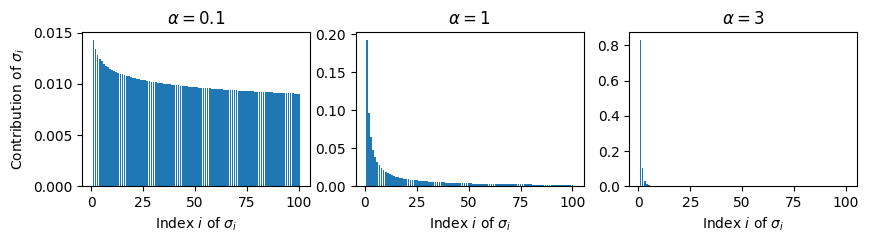
\includegraphics[scale=0.73]{plots/scew_dist.png}
\caption{Examples of how standard deviations are distributed according to 
zipf's law for different skewness levels ($\alpha$).} 
\end{figure}

So the needed parameters to describe a hypothetical are $\alpha$, $d$ the number of dimensions, and 
$n$ the number of points which is needed to decide the clipping probability.

I then calculated the expected error as described by equation 
\eqref{eq:Alg3Err2} denoting this as $\mathcal{E}_t$ and compare that to
\[
    \mathcal{E}_n = \lr{2C_n\sigma_{opt}}^2
\]
In which $C_n$ is choose as the minimal value satisfying 
$\prob{ \|x_i\|^2 > C_n^2} \le \frac{1}{n}$. 
I then calculate the fraction $\frac{\mathcal{E}_n}{\mathcal{E}_t}$ to compare 
the expected errors, and as I have $\sigma_{opt}^2$ in both the denominator and the numerator I 
can ommit caluclating this as doing so is not a trivial task. 
Figure \ref{fig:result} shows calculating this fraction for varying $\alpha \in [10^{-2}, 10^2]$, and for 
$d \in \{10, 100, 1000\}$ and $n \in \{10^2, 10^3, 10^6\}$.
It shows that when few dimensions have much more variance than the rest,
performing the transformation improes the expected error, for all 
configurations of $n$ and $d$.
\begin{figure}[h!]
\label{fig:result}
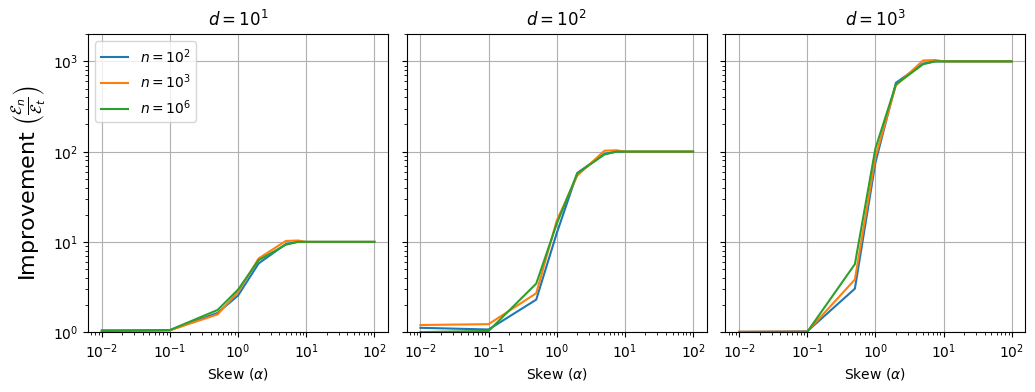
\includegraphics[scale=0.62]{plots/result.png}
\caption{Improvement of applying the transformation. 
Each subplot shows for a fixed number of dimensions $d$, how much the improvement is for different 
skewness paramters $\alpha$ and number of data points $n$,
 which is used to decide the clipping probability.}
\end{figure}



More generally it seems as though $n$ has no impact on the improvement of the method, 
which is not trivial as the clipping probability is chosen as $\frac{1}{n}$. 
It could perhaps have been that the transformation changed the distribution in such a way
that the tail was much longer.
Interestingly I observe that the method improves by a factor of $[1,d]$ 
quite like how the Elliptical Gaussian Mechanism improves the Gaussian Mechanism by a 
factor of $[1,d)$. Perhaps a similiar argument could be made in this case, 
if the distribution of the norms had a closed form or more analysis of it was done.
But the emperical evidence is quite strong in favor of this phenomenon being present here as well.




In this setting To create these hypothetical dataset, I 


in expected error by calculating 
%- Zipf's law for different amount of skewness of standard deviation
%- 10^-1 basically uniform and 10^1 basically only 1 dimension has variance
%- Introduce how results are shown
%- Skewness has great impact on improvement
%- improvement of [1, d] just like original paper (and ref the equation)
% In the future:
%- Comparison to state of the art methods, including the clipping bias.
\todo{Downside of not creating dataset adn doing algo is that clipping bias is not taken into account}
\todo{Compare method to state of the art on hypothetical datasets.}
\todo{Mention that method requires sigmas to be known as estimating would take up most of
the privacy budget.}


\section{Discussion \& Future work}
% On the problem setup
Earlier when I defined the problem at hand I also defined the constraint that the expected norm after 
transforming the data should be 1, i.e. the constraint given by equation \eqref{eq:normcon}. 
This constraint is perhaps not optimal in terms of how the problem should be restricted. The idea behind the constraint
is to force the data to become more symmetrical in the transformed space, however it does not necessarily enforce this. 
An alternative constraint which I initially investigated for this project was to find a transformation, such that the majority of 
data entries lie within a ball with diameter 1, and entries outside would be clipped.
In this transformed space it would be sufficient to add noise drawn from
$\mathcal{N}(0, \sigma_{opt}^2)$. The constraint would thus be the following
\begin{equation}
\label{eq:AltCon}
    \prob{ \| x_i \odot \bm{b} \| > \frac{1}{2}} \le \frac{1}{n} 
\end{equation}
To achieve optimal results with this constraint it would be required to know the cumulative density function of $\| x_i \odot \bm{b} \|$, 
which as discussed earlier is distributed as a generalized chi square and does not have a closed form. 
So without a closed form there would be no way of finding optimal values for $b_j$. 
Another option would be to have the same constraint, but instead define it in terms of a tail inequality such as the one
given by lemma \ref{lem:Bernstein}. However the constraint on $t$ in that lemma can be quite restrictive for some inputs, 
and the method would not be applicable to all datasets.
I also attempted to find optimal values for $b_j$ whilst using Chebyshev's inequality to give closed forms for equation \eqref{eq:AltCon}, 
unfortunately this lead to a very complicated optimization problem, which I did not attempt to solve.
The benefit os using Chebyshev's inequality would be that it is very generalized and would be applicable to any dataset, 
but it is also quite well known that the bounds given by Chebyshev's inequality are usually quite loose. 
I settled for the constraint where the expected norm is $1$, which intuitively seemed quite good and was much easier to solve. 
The emperical data also support this intuition \\

% On the empirical evaulation
% downside of not creating dataset and actually doing the algo
% is that clipping bias is not taken into account
In the emperical evaluation of the method I chose to compare the method
to that which I deemed the most natural thing to do if 
one were to use the Gaussian Mechanism. Simply clip points with 
probability $\frac{1}{n}$, and add noise according to this.
This method nor doing it with a transformation does take into account
the bias which comes from clipping the data in the first place.
And preferably Algorithm \ref{alg:EGM2} (doing the transformation) should
be compared to state of the art methods, such as the ones in \cite{coinpress, Huang2021}.
In such as comparison the clipping bias should be taken into account as well, and
in a more in depth analysis of the Algorithm \ref{alg:EGM2} it
would interesting to investigate the bias-variance tradeoff and finding an
optimal clipping probability $p_{C}$.


\subsection{Limitation}
The biggest limitation of the method proposed in this project, is the requirement for an estimate
of the mean $\bm{\mu}$ as this is a problem equivalent to the one which the mechanism proposed here solves.
The desire is that incorporating this is possible, as other methods in recent research has achieved something similair.
Many parallels can be drawn to \cite{Huang2021}, as they also clip points
according to some sphere in which they privately find a center for the sphere. The main concept which is introduced in this project
is the noise is added to each dimension as a function of its variance, which is not done in \cite{Huang2021}.
My hope is that the analysis presented here is of value in a context where finding the center of the sphere is incorporated
into the mechanism itself.

\newpage
\section{It is a mess, don't look here}
\subsection{Gaussian data}
Let $X^{(j)} \sim \mathcal{N}(0, \sigma_j^2)$ 
As the expected $l_2$-norm of $x_i$ is given by
\[
    \ee{x_i} = \sum_{j=1}^d \sigma_j^2
\]
To achieve an expected norm of $1$ I will scale 
each dimension by a factor $\frac{1}{b_j}$ which achieves this.
If 
\[
\hat{x_i} = \left( \frac{x_i^{(0)}}{b_0}, \frac{x_i^{(1)}}{b_1}, \dots, \frac{x_i^{(d)}}{b_d} \right)
\]
This means that $X^{(j)} \sim \mathcal{N}(0,\frac{\sigma_j^2}{b_j^2})$ 
and the expected norm is given by 
\[
    \ee{x_i} = \sum_{j=1}^d \frac{\sigma_j^2}{b_j^2}
\]
and I can introduce that constraint that the expected norm
after the transformation should be $1$.
In such a case when noise is added after the transformation
$\hat{X} + \eta$
where $\eta \sim N(0, t^2)$ and achieves \edp in this space
then then due to linearity of transformation the noise 
introduced in the original space is then given by
then the error is





I desire a transformation of $x_i^{(j)}$ such that the 
expected norm is $1$. Thus I must scale each dimension by
$\frac{1}{b_j}$, and have that 
\[
    \ee{x_i} = 1
\]

Minimize $\| \hat{\eta} \|$ under the constraint that $\ee{x_i} = 1$  

\begin{lemma}
\label{lem:chibound}
Let $X \sim \mathcal{N}(0,\sigma^2)$, and $\Phi$ denote the 
cumulative density function of $\mathcal{N}(0,1)$, then the 
cumulative density function of $X^2$ is given by
\[
    F_{X^2}(x) = \prob{X^2 \le x} = 2\Phi \lr{\frac{\sqrt{x}}{\sigma}} - 1
\]
\end{lemma}
\begin{proof}
\begin{align*}
    &\prob{X^2 \le x} =
    \prob{ |X| \le \sqrt{x}} =
    2 \prob{0 \le X \le \sqrt{x}}  \\
    & =2  \lr{\prob{X \le \sqrt{x}} - \prob{X \le 0}} =
    2 \lr{\prob{X \le \sqrt{x}} - \frac{1}{2}}  \\
    &= 2 \Phi \lr{\frac{\sqrt{x}}{\sigma}} - 1 
\end{align*}
\end{proof}
\begin{corollary}
From lemma \ref{lem:chibound} we can give following bound for $X \sim \mathcal{N}(0,\sigma^2)$.
\[
    \prob{X^2 > (4\sigma)^2} < 10^{-4}
\]
\end{corollary}


\newpage





Bernsteins inequality then states that
\[
    \prob{\sum_{j \in [d]} X_j \ge 2 t \sqrt{ \sum_{j \in [d]} \Exp{X_i^2}}} < e^{-t^2}
\]
for all 
\[
    0 \le t \le \frac{1}{2L} \sqrt{\sum}
\]

I have that $\bar{X}$ is a standard gaussian variable. \\
Let $Y_j = X_j^2$ I am interested in $\sum_{j \in [d]} Y_j$,
then it has 
\begin{align*}
    &\Exp{ |Y_j^k| } = \Exp{ |X_j^{2k}| } = \Exp{ |X_j|^{2k} } = 
    \Exp{ | \sigma_j \bar{X} |^{2k} } = \\
    &| \sigma_j |^{2k} \Exp{ | \bar{X} |^{2k}} = 
    \sigma_j ^{2k} \prod_{c=1}^k 2c = \sigma_j^{2k} \cdot 2^k \cdot k!
\end{align*}
Which means $\Exp{Y_j^2} = 8 \sigma_j^{4}$.
To check the constraint (find value for L)
\begin{align*}
    &\sigma_j^{2k} \cdot 2^k \cdot k! \le
    \frac{1}{2} \cdot 8 \sigma_j^{4} \cdot L^{k-2} k! \iff \\
    &\sigma_j^{2k} \cdot 2^k \le 4 \sigma_j^4 \cdot L^{k-2} \iff \\
    &\sigma_j^{2(k-2)} \cdot 2^k \le 4 \L^{k-2}
\end{align*}
We have that 
$\sigma_j = \sigma_j b_j = \frac{\sqrt{\sigma_j}}{\sqrt{\sum_{i \in [d]} \sigma_i}} = \sqrt{\frac{\sigma_j}{\sum_{i \in [d]} \sigma_i}}$.
Therefore
\begin{align*}
    &\sigma_j^{2(k-2)} \cdot 2^k  = 
    \lr{\sqrt{\frac{\sigma_j}{\sum_{i \in [d]}\sigma_i}}}^{2(k-2)} \cdot 2^k = \\
    &\lr{\frac{\sigma_j}{\sum_{i \in [d]}\sigma_i}}^{k-2} \cdot 2^k \le 2^k
\end{align*}
This therefore implies
\[
    2^k \le 4 L^{k-2} \iff
    2^{k-2} \le L^{k-2} \iff
    2 \le L
\]
If it is desired that less than $10^{-p}$ points are removed then 
$t = \sqrt{p \ln(10) }$ as long as 
\[
    \sqrt{p \ln(10)} \le \frac{1}{2L}\sqrt{\sum_{j \in [d]} \Exp{X_j^2}} 
    = \sqrt{4} \cdot \frac{\sqrt{\sum_{i \in [d]} \sigma_i^2}}{\sum_{i \in [d]} \sigma_i}
\] 



\paragraph*{An alternative}
Again minimize $\| \hat{\eta} \|$, but instead the constraint
comes from Chebyshev's inequality, I always have that
\[
    \prob{ |\|x_i\|^2 - \ee{x_i}| \ge k \cdot \sqrt{\var{\|x_i\|^2}}} \le \frac{1}{k^2}
\]
Therefore I can set $\frac{1}{k^2} = 0.05$, and find a 
transformation where I decide how many standard deviations
I must be away from the mean to have norm greater than 1, i.e.
\begin{align*}
    \ee{x_i} + k \cdot \sqrt{\var{\|x_i\|^2}} = 1 \implies k = \frac{1-\ee{x_i}}{\sqrt{\var{\|x_i\|^2}}}
\end{align*}
I then have that
\[
    \frac{1}{k^2} = \frac{1}{\lr{\frac{1-\ee{x_i}}{\sqrt{\var{\|x_i\|^2}}}}^2} = 
    \lr{\frac{\sqrt{\var{\|x_i\|^2}}}{1-\ee{x_i}}}^2 = 
    \frac{\var{\|x_i \|^2}}{\lr{1 - \ee{x_i}}^2}
\]
I already know that
\begin{alignat*}{2}
    &\ee{x_i} = &\sum_{j=1}^d \frac{\sigma_j^2}{b_j^2} \\
    &\var{\|x_i \|^2} = 2 &\sum_{j=1}^d \frac{\sigma_j^4}{b_j^4}
\end{alignat*}
I therefore have the constraint 
\[
    \frac{\var{\|x_i \|^2}}{\lr{1 - \ee{x_i}}^2} = 
    \frac{2 \sum_{j=1}^d \frac{\sigma_j^4}{b_j^4} \\}
    {\lr{1-\sum_{j=1}^d \frac{\sigma_j^2}{b_j^2} }^2} = 
    0.05
\]
Be aware that this could find cases where expected norm is greater than 1
and the constraint then says that they are never less than 1 in norm.
Another restriction could be that expected norm is < 1.

Chebyshev's inequality could also be used when expected norm should be 1
and then put a bound on number of std away one must be to have less than 
0.05 fraction of data removed.

\newpage


\newpage

\section*{Extra}
Determining $\alpha$ using Bernsteins inequality
\[
    \prob{\|x_i\|^2 - \ee{x_i} > t} < 2 \cdot \exp \lr{- \frac{t^2/2}{\var{\|x_i\|^2} + C \cdot t/3}}
\]
In the case where $\ee{x_i} = 1$ and $b_i$ is optimized in this case,
we have that
\begin{align*}
    &P(\|x_i\|^2 > 1 + t) < 2 \exp \lr{- \frac{t^2/2}{\var{\|x_i\|^2} + C \cdot t/3}} \\
    &\var{\| x_i \|^2} = 2 \frac{\sum_i^d \sigma_i^2}{\lr{\sum_i^d \sigma_i}^2} \\
    &C = \max_{i \in [d]} \lr{\sigma_i} \cdot \frac{16}{\sum_i^d \sigma_i}
\end{align*}
$C$ is decided such that less than $0.0001$ fraction of the data is outside this bound
in each dimension. i.e. 
\[
    \forall j \in [d] \text{ : }\prob{X^{(j)} > C} < 0.0001
\]

Solving for $t$
\begin{align*}
&2 \cdot \exp \lr{- \frac{t^2/2}{\var{\|x_i\|^2} + C \cdot t/3}} = 0.0001
\iff \ln(\frac{0.0001}{2}) = -\frac{t^2/2}{\var{\|x_i\|^2} + C \cdot t/3}
\implies \\ &t = - \frac{C \ln(\frac{0.0001}{2}) - 
\sqrt{\ln(\frac{0.0001}{2})(-18 \cdot \var{\|x_i\|^2} + C^2\ln(\frac{0.0001}{2}))}}{3}
\end{align*}
Then we have that $\alpha = 1 + t$.

\todo{Determine $\alpha$ for the bound using \url{https://en.wikipedia.org/wiki/Concentration_inequality}, or \url{https://web.stanford.edu/class/cs229t/2017/Lectures/concentration-slides.pdf}}


\bibliography{refs.bib}{}
\bibliographystyle{acm}


\end{document}

